\section{Recommendations for Run 2 b-taggers}

\subsection{High level taggers: DL1 series}

\begin{figure}[htbp]
  \centering
  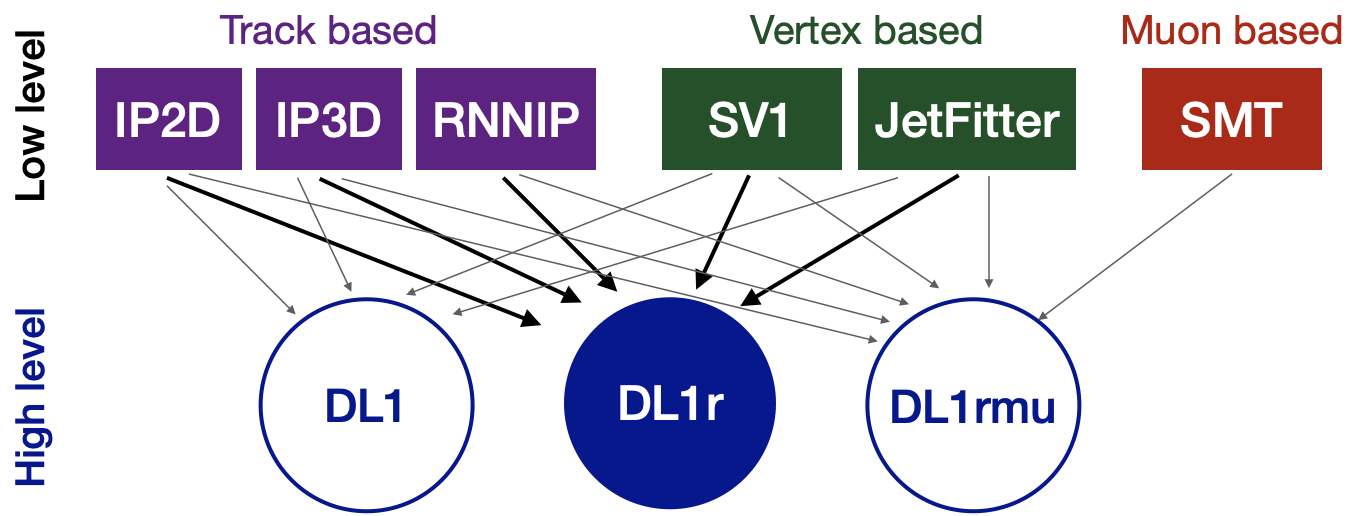
\includegraphics[width=\textwidth]{figures/ftag/ATLAS-taggers-all}
  \caption{The high level taggers that compared in the Run 2 analysis optimization.}
  \label{fig:ATLAS-taggers-all}
\end{figure}


% PFlow + VR results

% links
% http://atlas.web.cern.ch/Atlas/GROUPS/PHYSICS/PLOTS/FTAG-2019-005/
% http://atlas.web.cern.ch/Atlas/GROUPS/PHYSICS/PLOTS/FTAG-2019-006/

\foreach \jetdef in {PFlow,VR}{
   
    \subsection{\jetdef \ trainings}
    \def\figpath{figures/ftag/\jetdef \ trainings}
    
    \begin{figure}[htbp]
        \centering
        % light
        \subfloat[]{ 
                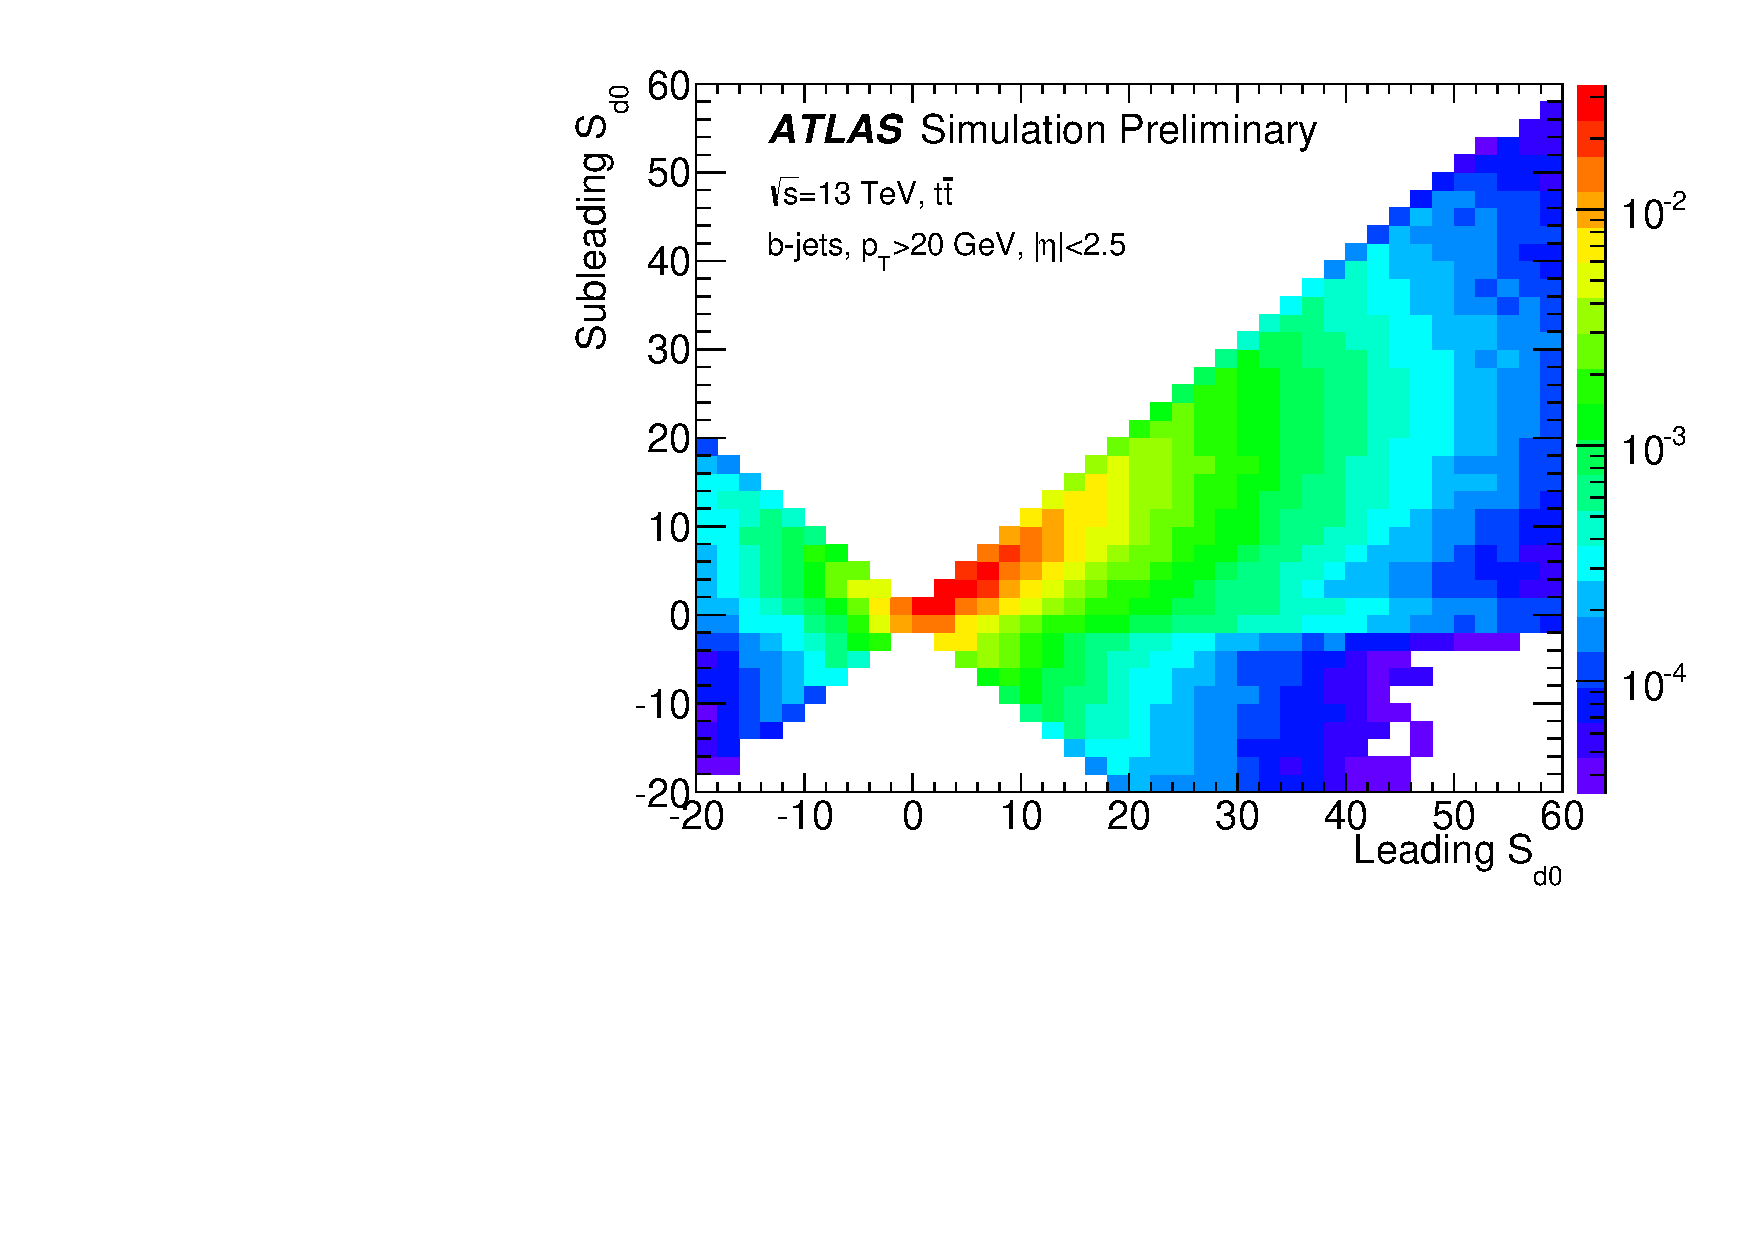
\includegraphics[width=0.48\linewidth]{\figpath/fig_01a}
        } 
         \subfloat[]{ 
                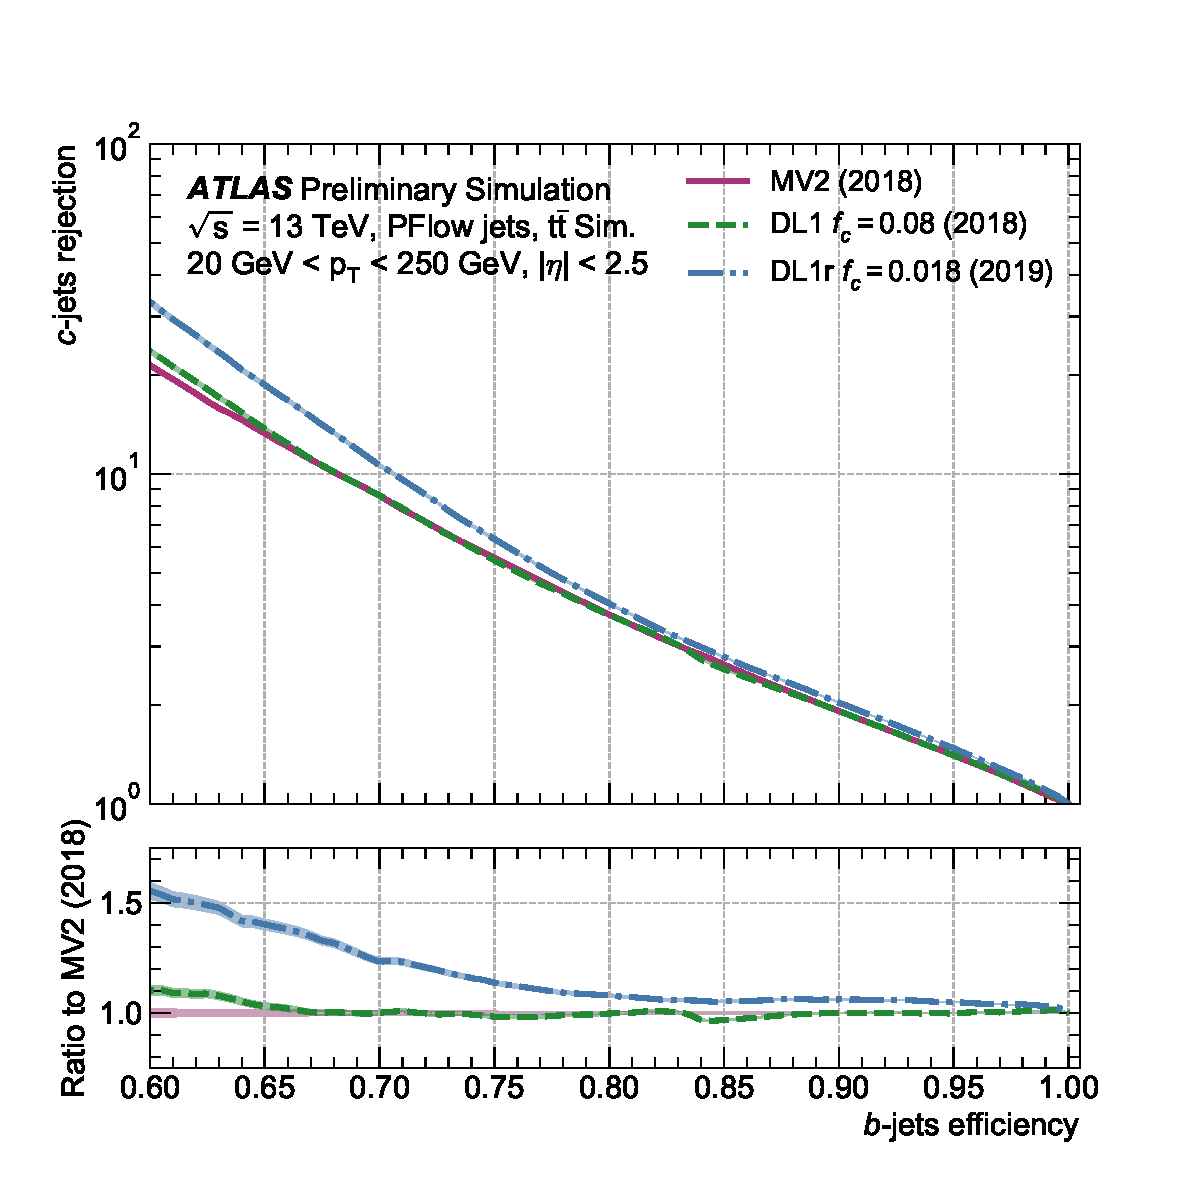
\includegraphics[width=0.48\linewidth]{\figpath/fig_01b}
        } 
        \caption{}
        \label{fig:\jetdef-fig1}
    \end{figure}
    
    \begin{figure}[htbp]
        \centering
        % light
        \subfloat[]{ 
                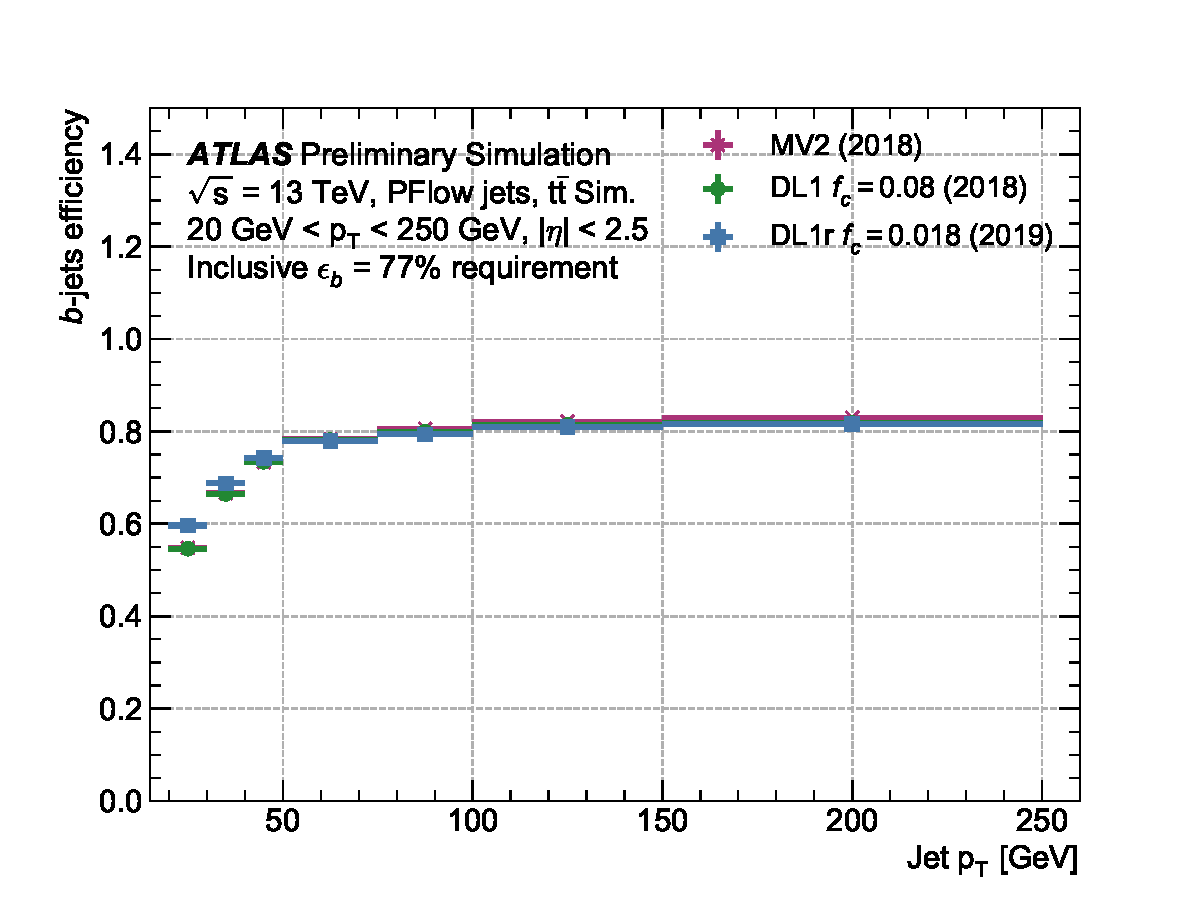
\includegraphics[width=0.33\linewidth]{\figpath/fig_02a}
        } 
         \subfloat[]{ 
                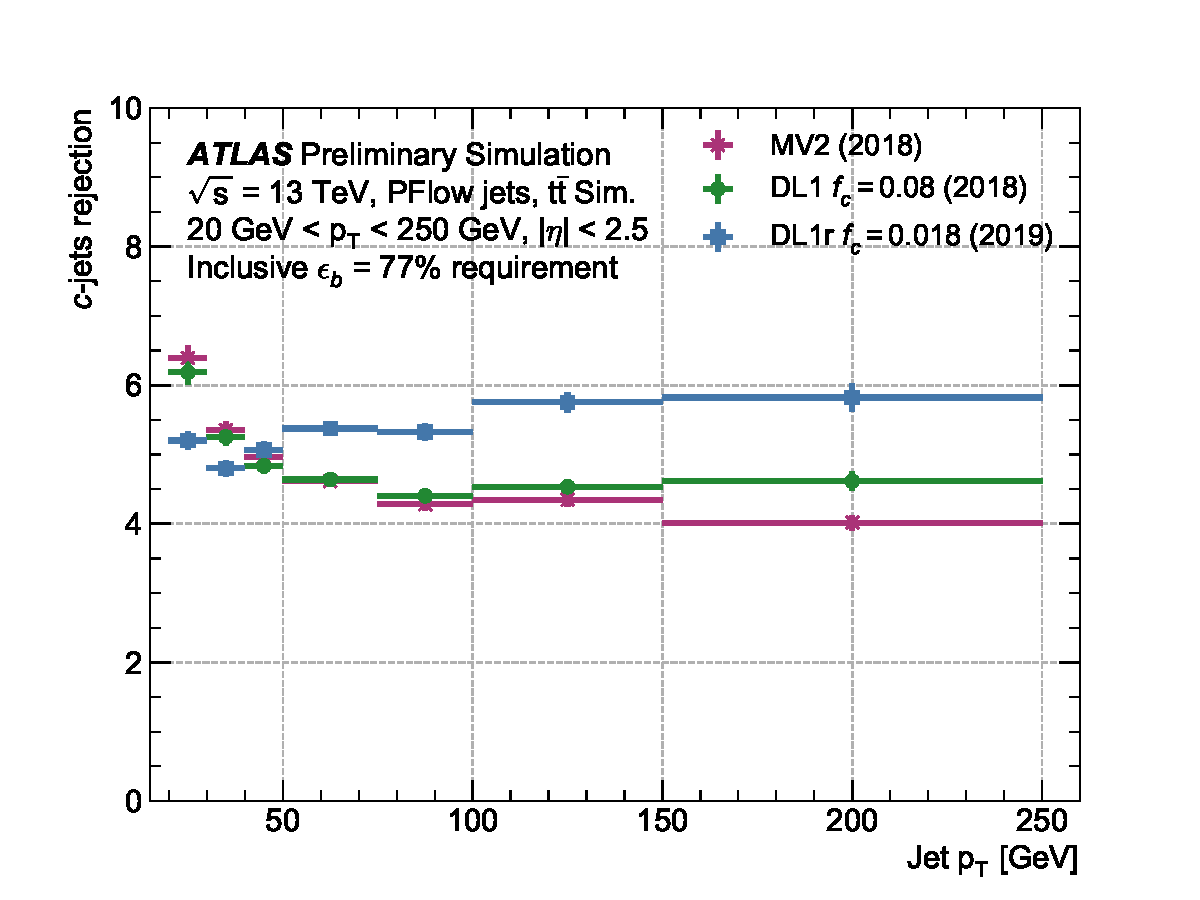
\includegraphics[width=0.33\linewidth]{\figpath/fig_02b}
        } 
        \subfloat[]{ 
                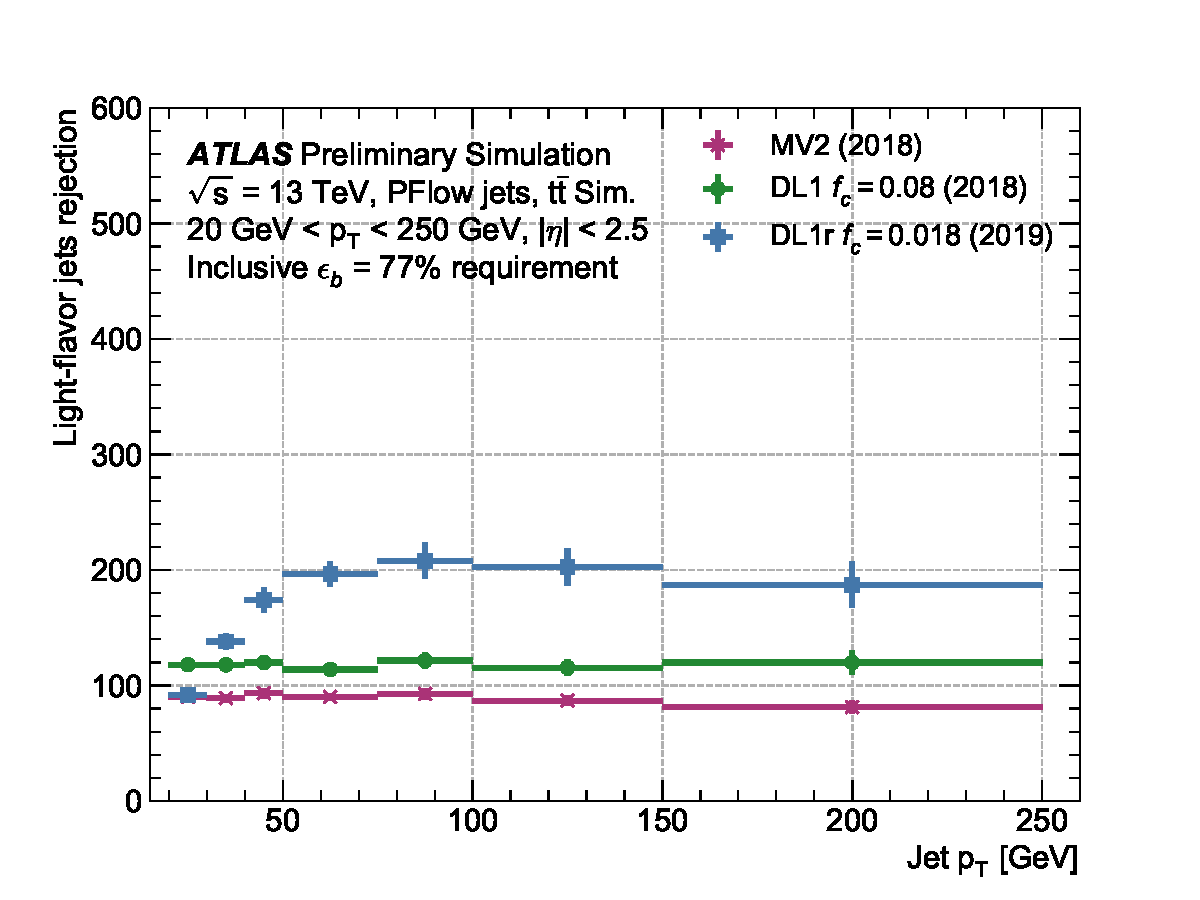
\includegraphics[width=0.33\linewidth]{\figpath/fig_02c}
        } 
        \caption{}
        \label{fig:\jetdef-fig2}
    \end{figure}
    
    \begin{figure}[htbp]
        \centering
        % light
        \subfloat[]{ 
                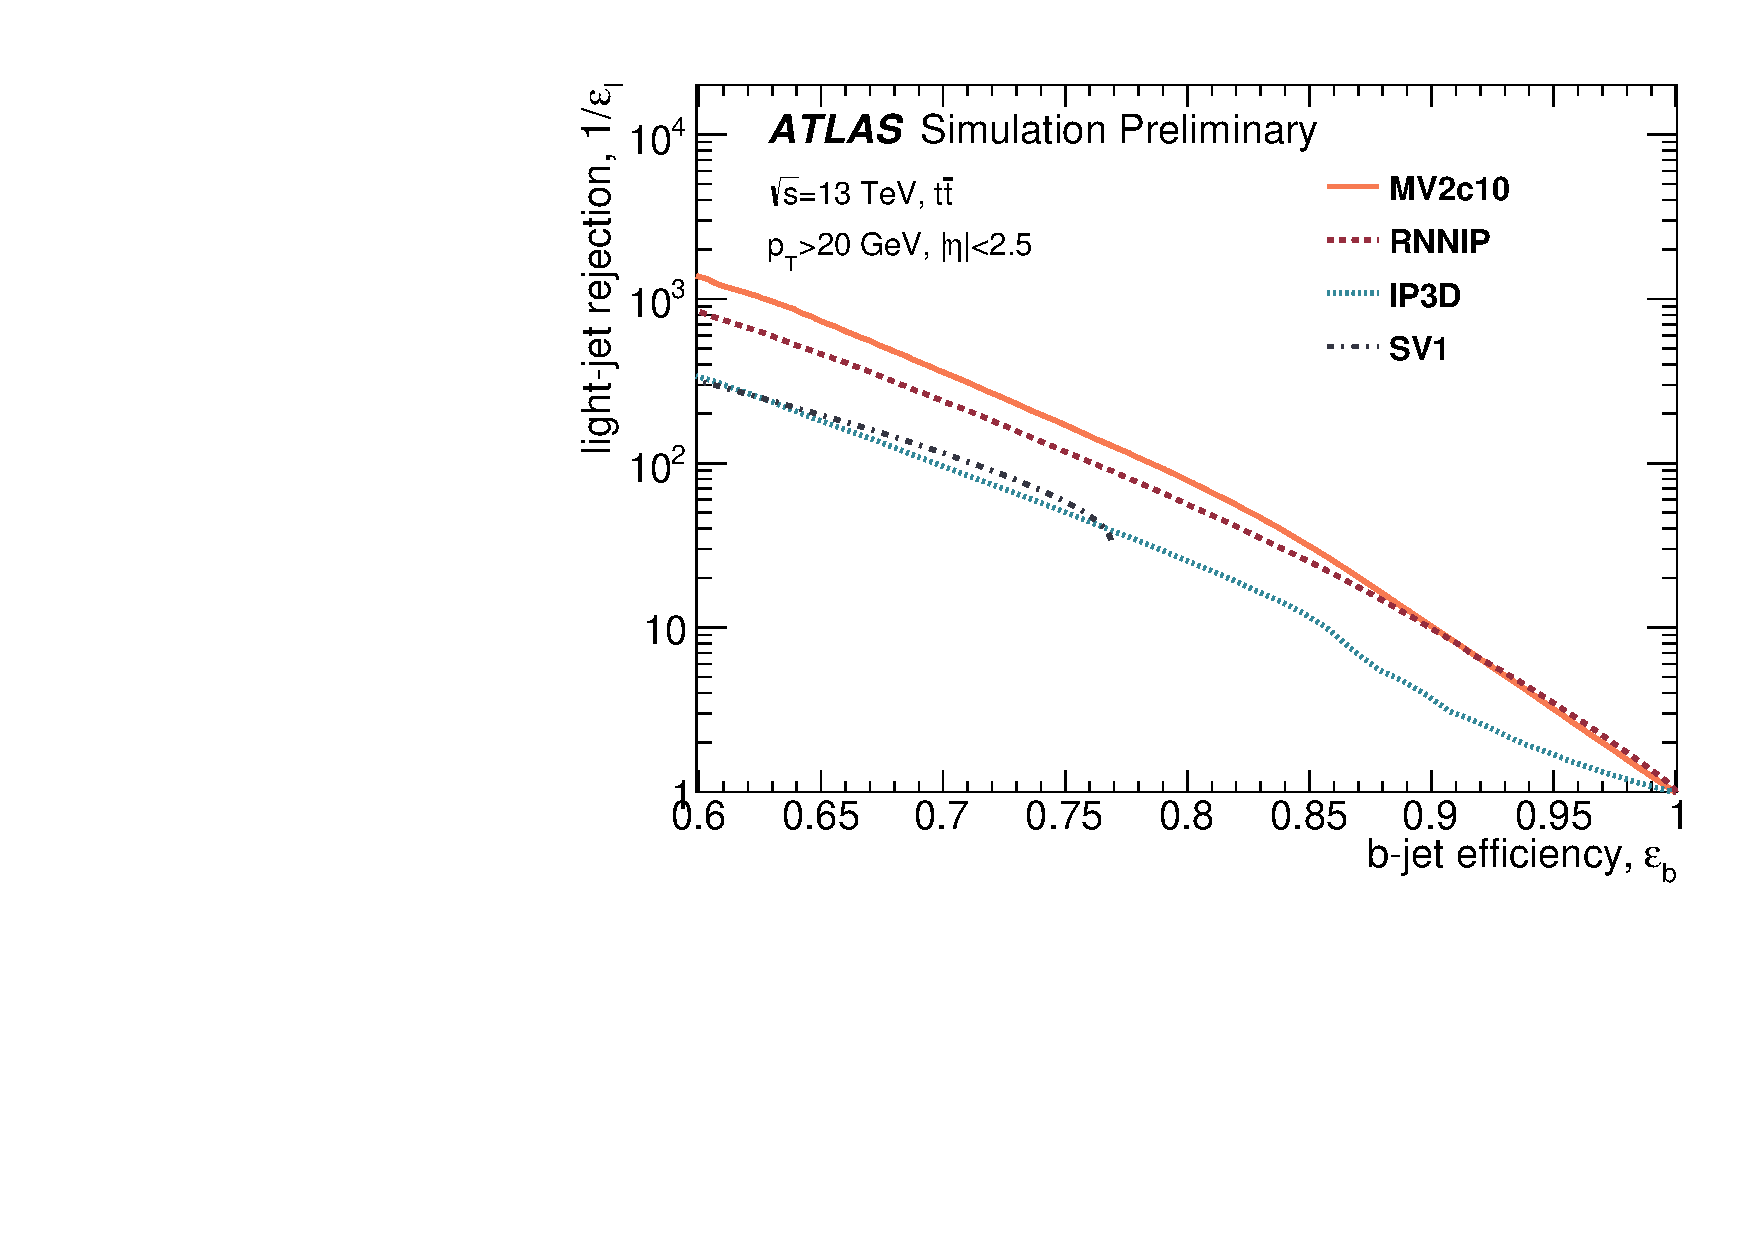
\includegraphics[width=0.48\linewidth]{\figpath/fig_03a}
        } 
         \subfloat[]{ 
                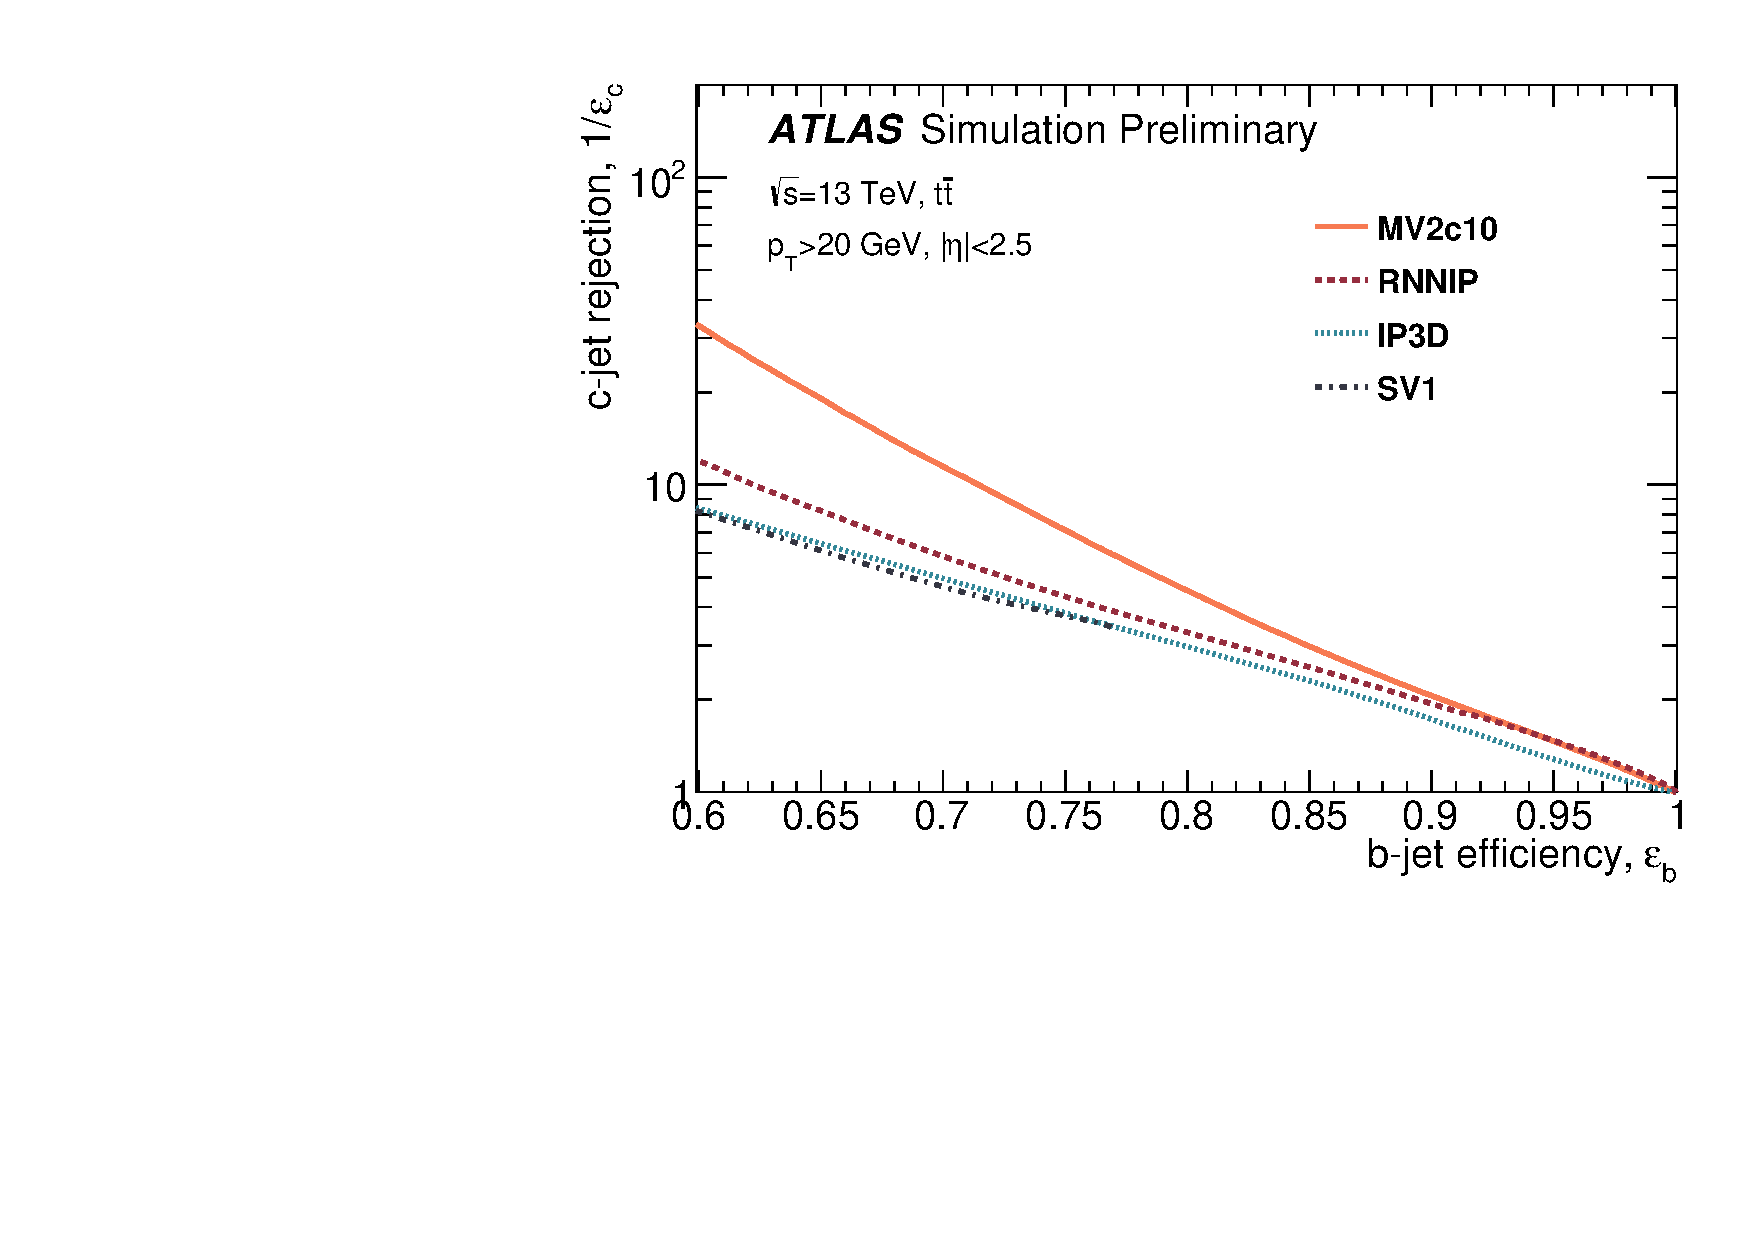
\includegraphics[width=0.48\linewidth]{\figpath/fig_03b}
        } 
        \caption{}
        \label{fig:\jetdef-fig3}
    \end{figure}
    
    \begin{figure}[htbp]
        \centering
        % light
        \subfloat[]{ 
                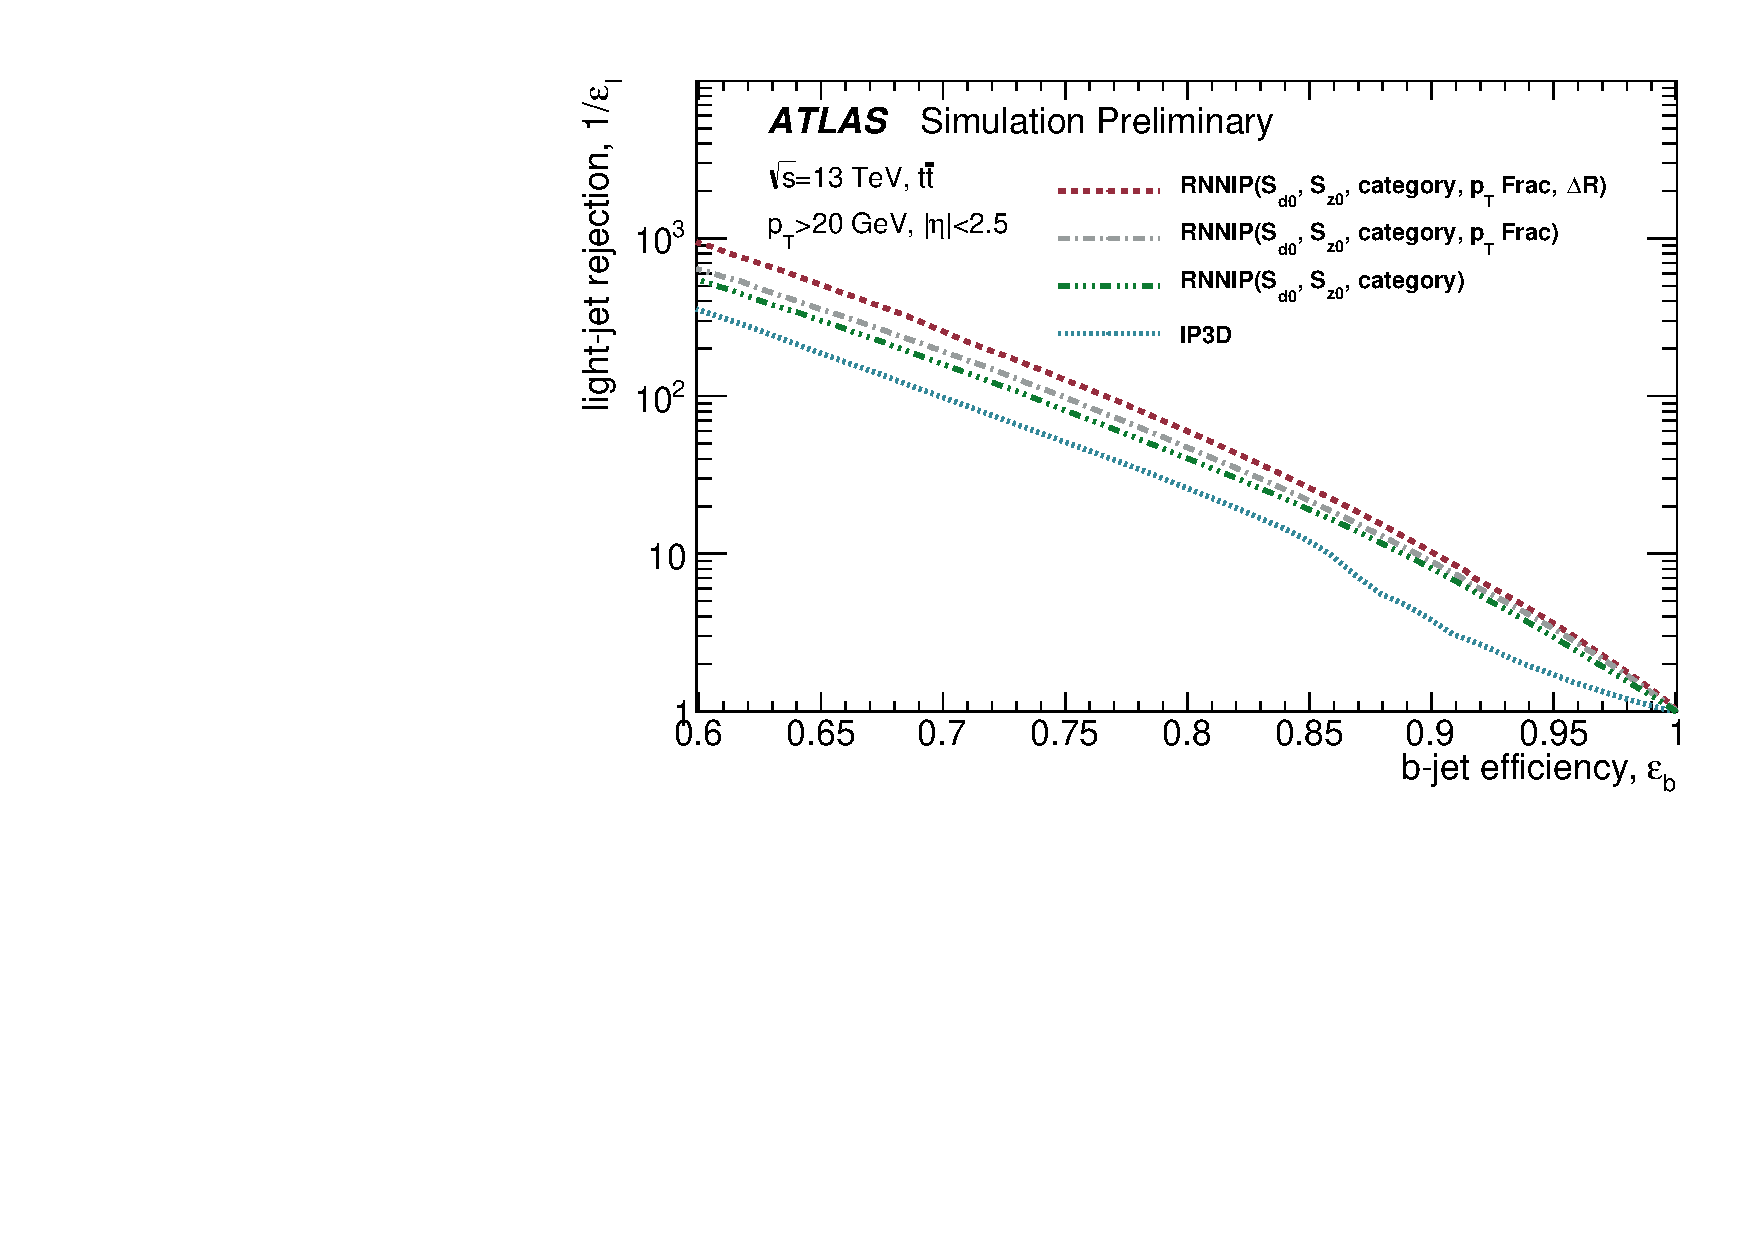
\includegraphics[width=0.48\linewidth]{\figpath/fig_04a}
        } 
         \subfloat[]{ 
                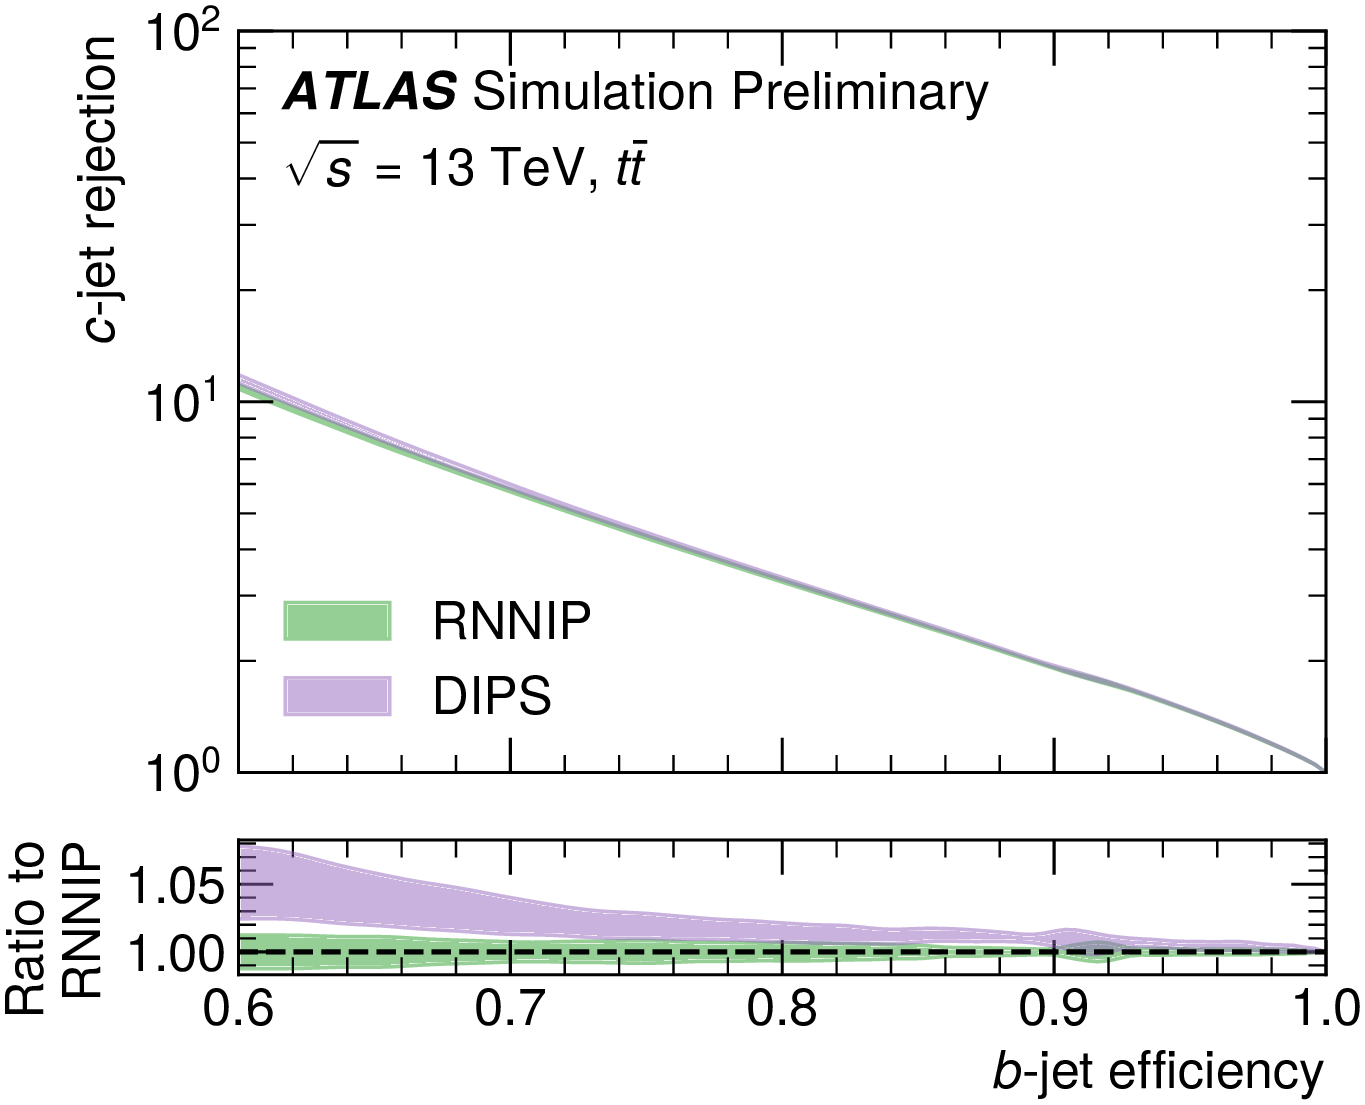
\includegraphics[width=0.48\linewidth]{\figpath/fig_04b}
        } 
        \caption{}
        \label{fig:\jetdef-fig4}
    \end{figure}
    
    \begin{figure}[htbp]
        \centering
        \subfloat[]{ 
                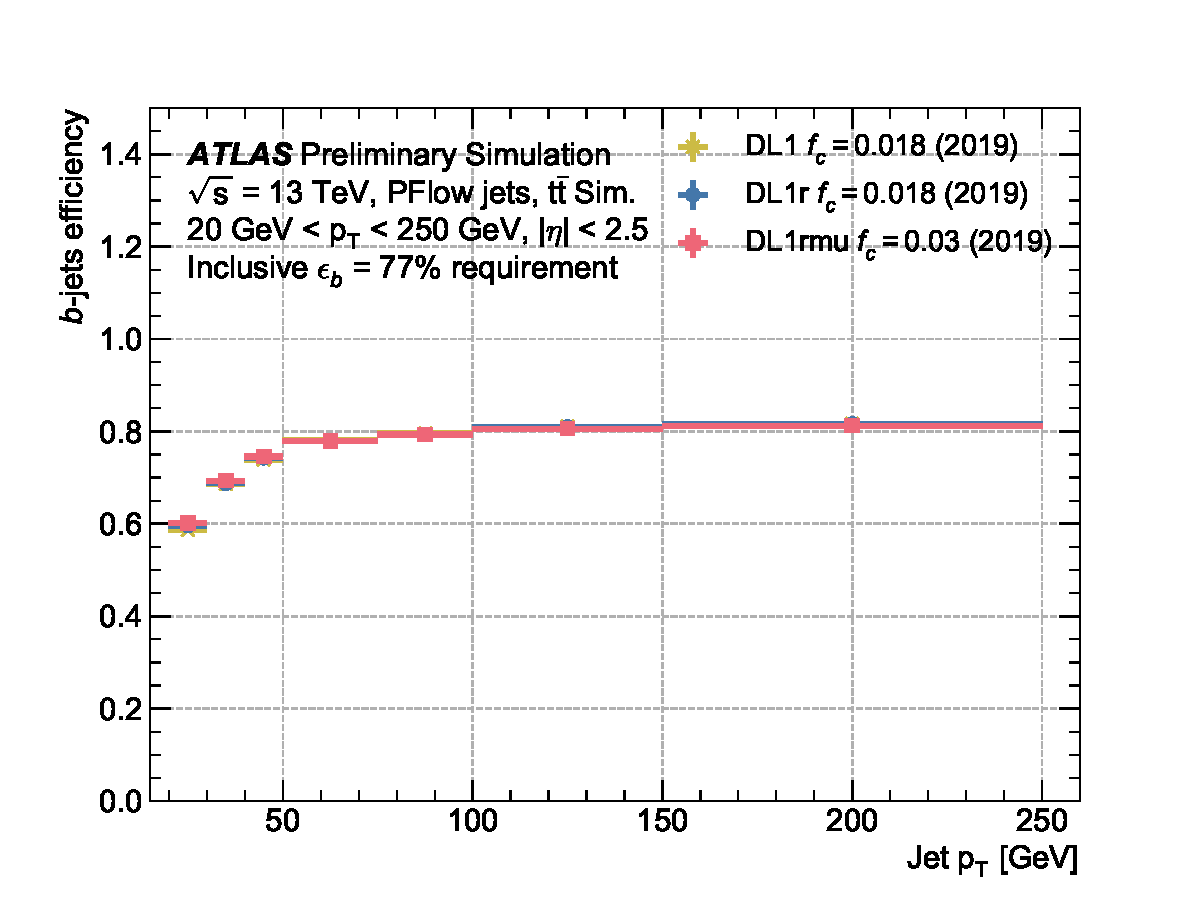
\includegraphics[width=0.33\linewidth]{\figpath/fig_05a}
        } 
         \subfloat[]{ 
                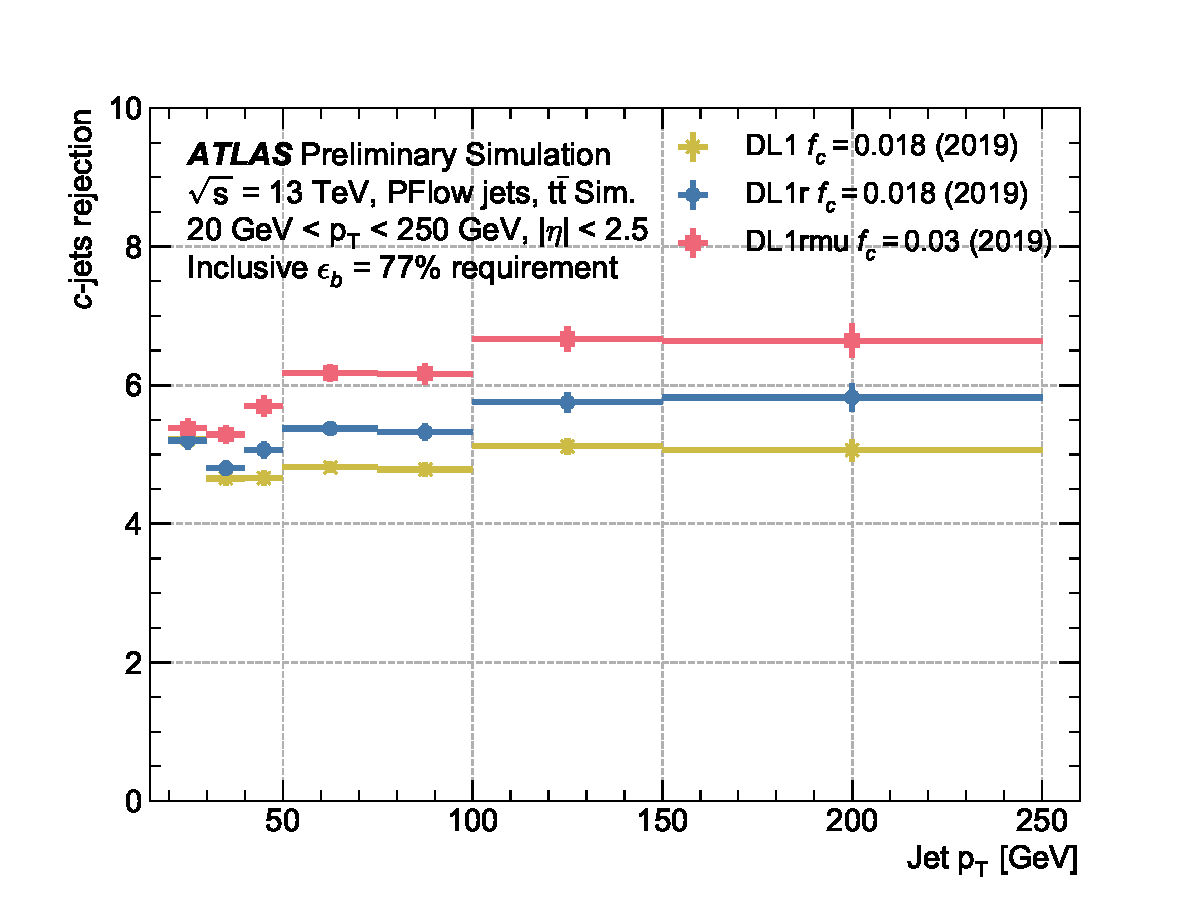
\includegraphics[width=0.33\linewidth]{\figpath/fig_05b}
        } 
         \subfloat[]{ 
                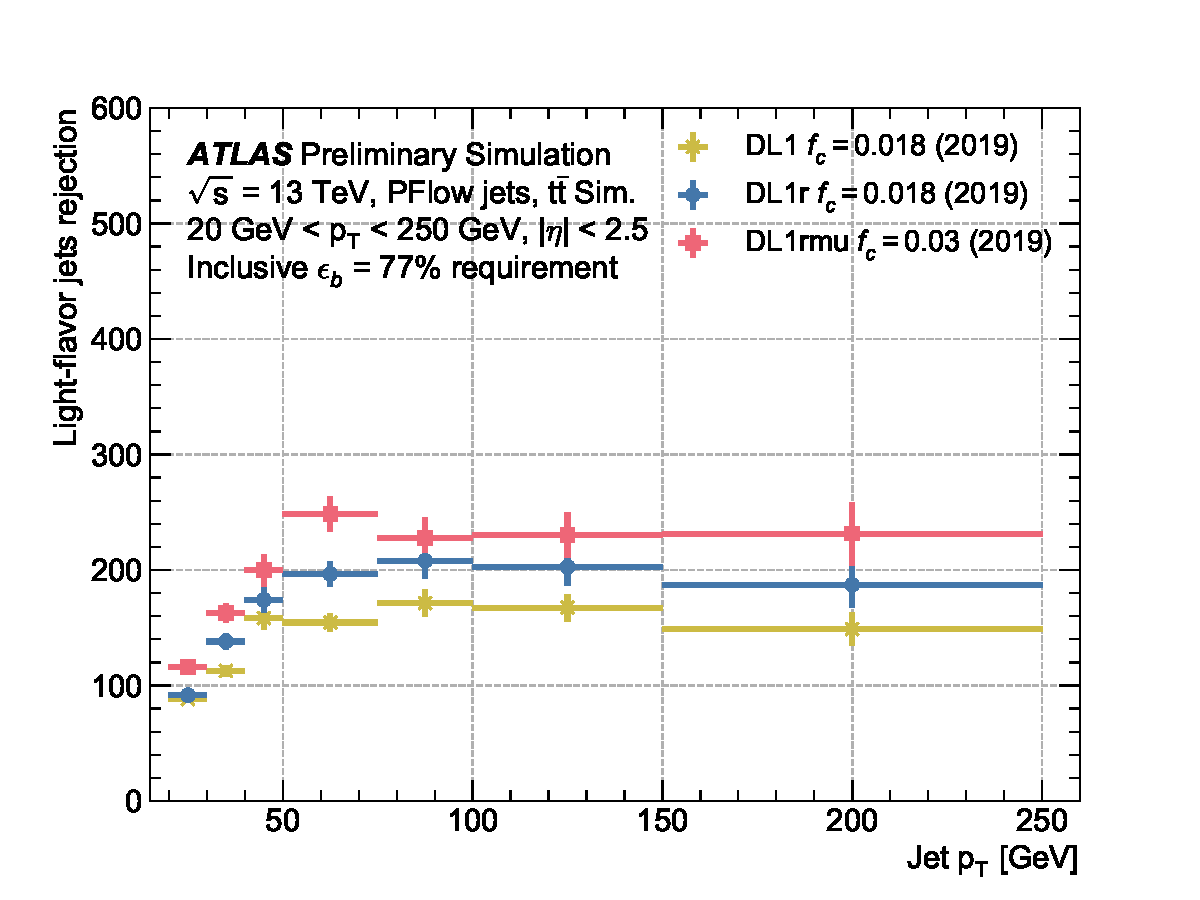
\includegraphics[width=0.33\linewidth]{\figpath/fig_05c}
        } 
        \caption{}
        \label{fig:\jetdef-fig5}
    \end{figure}

%   DL1rmu with the flat eff WP - less useful  
%    \begin{figure}[htbp]
%        \centering
%        \subfloat[]{ 
%                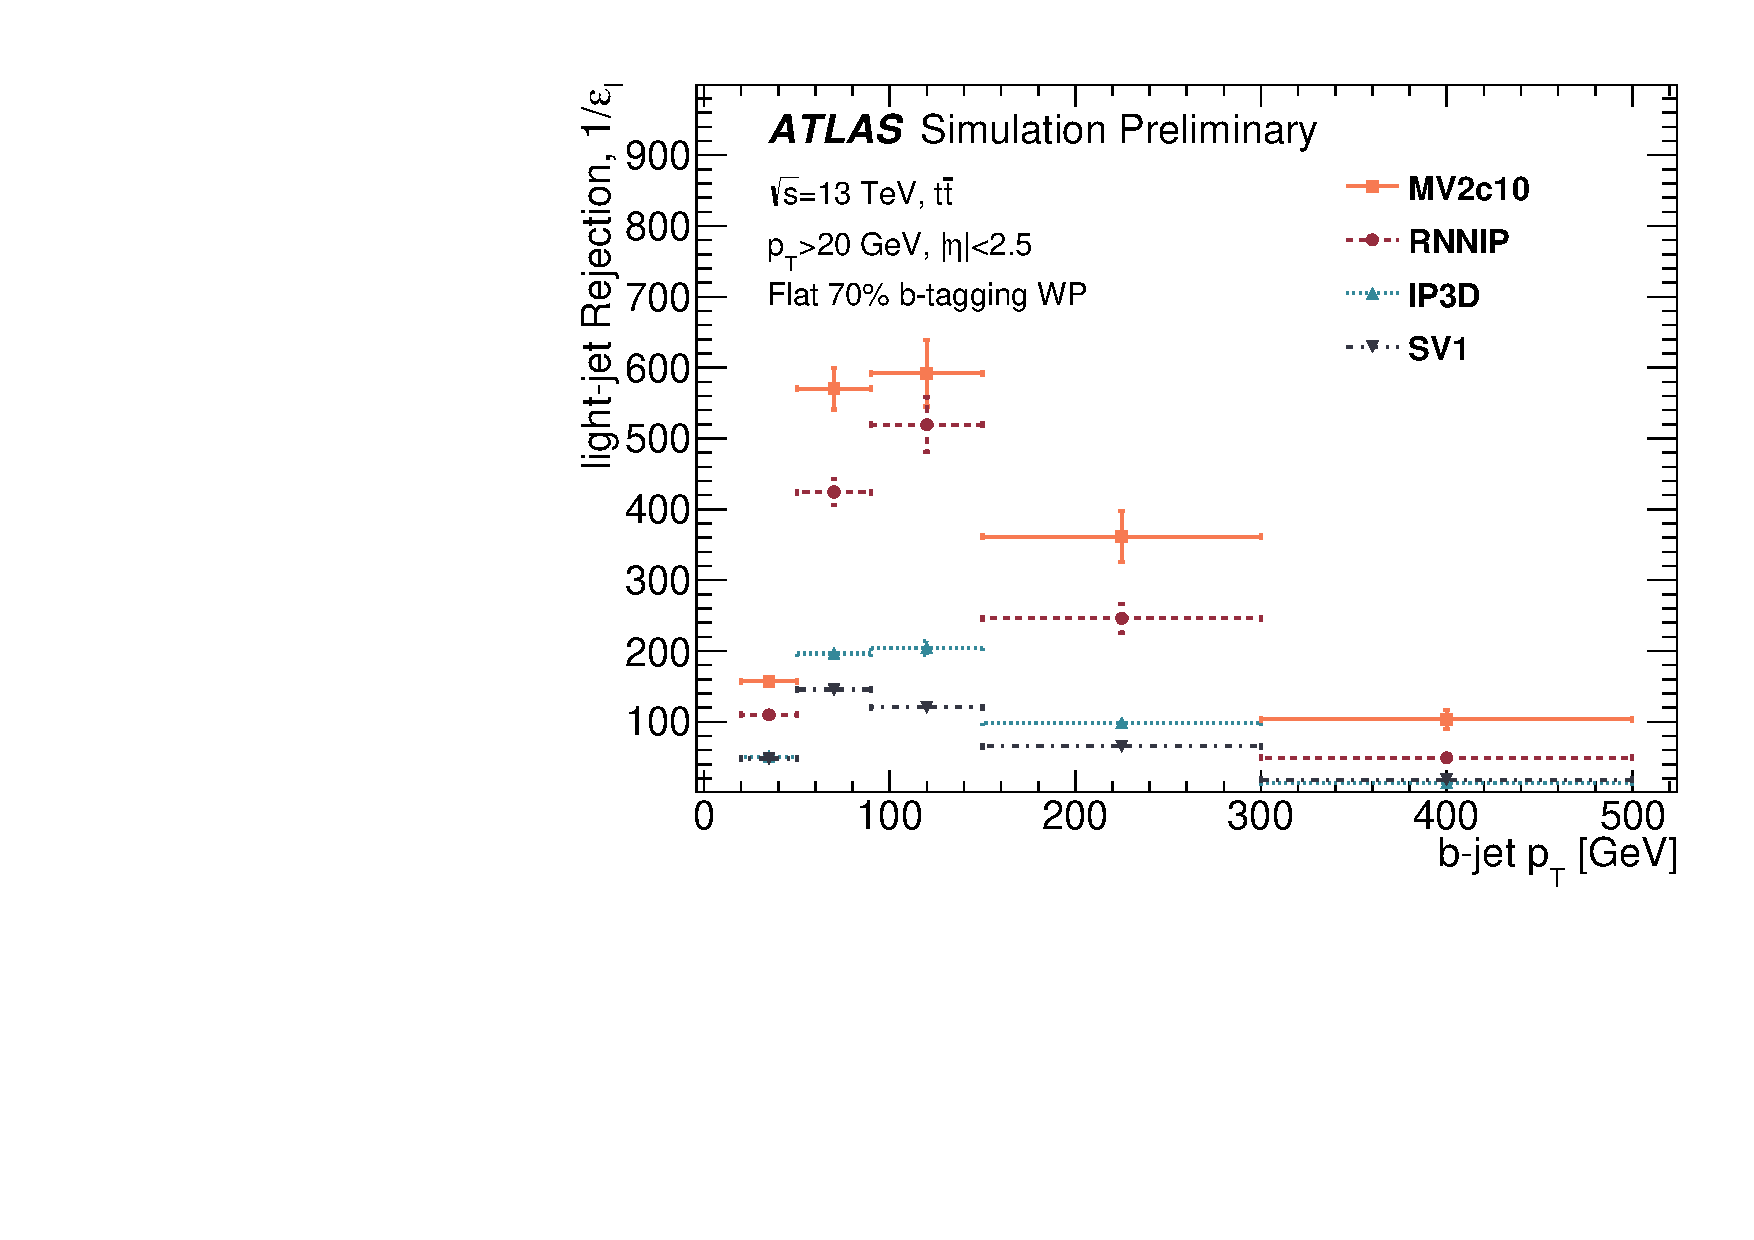
\includegraphics[width=0.41\linewidth]{\figpath/fig_06a}
%        } 
%         \subfloat[]{ 
%                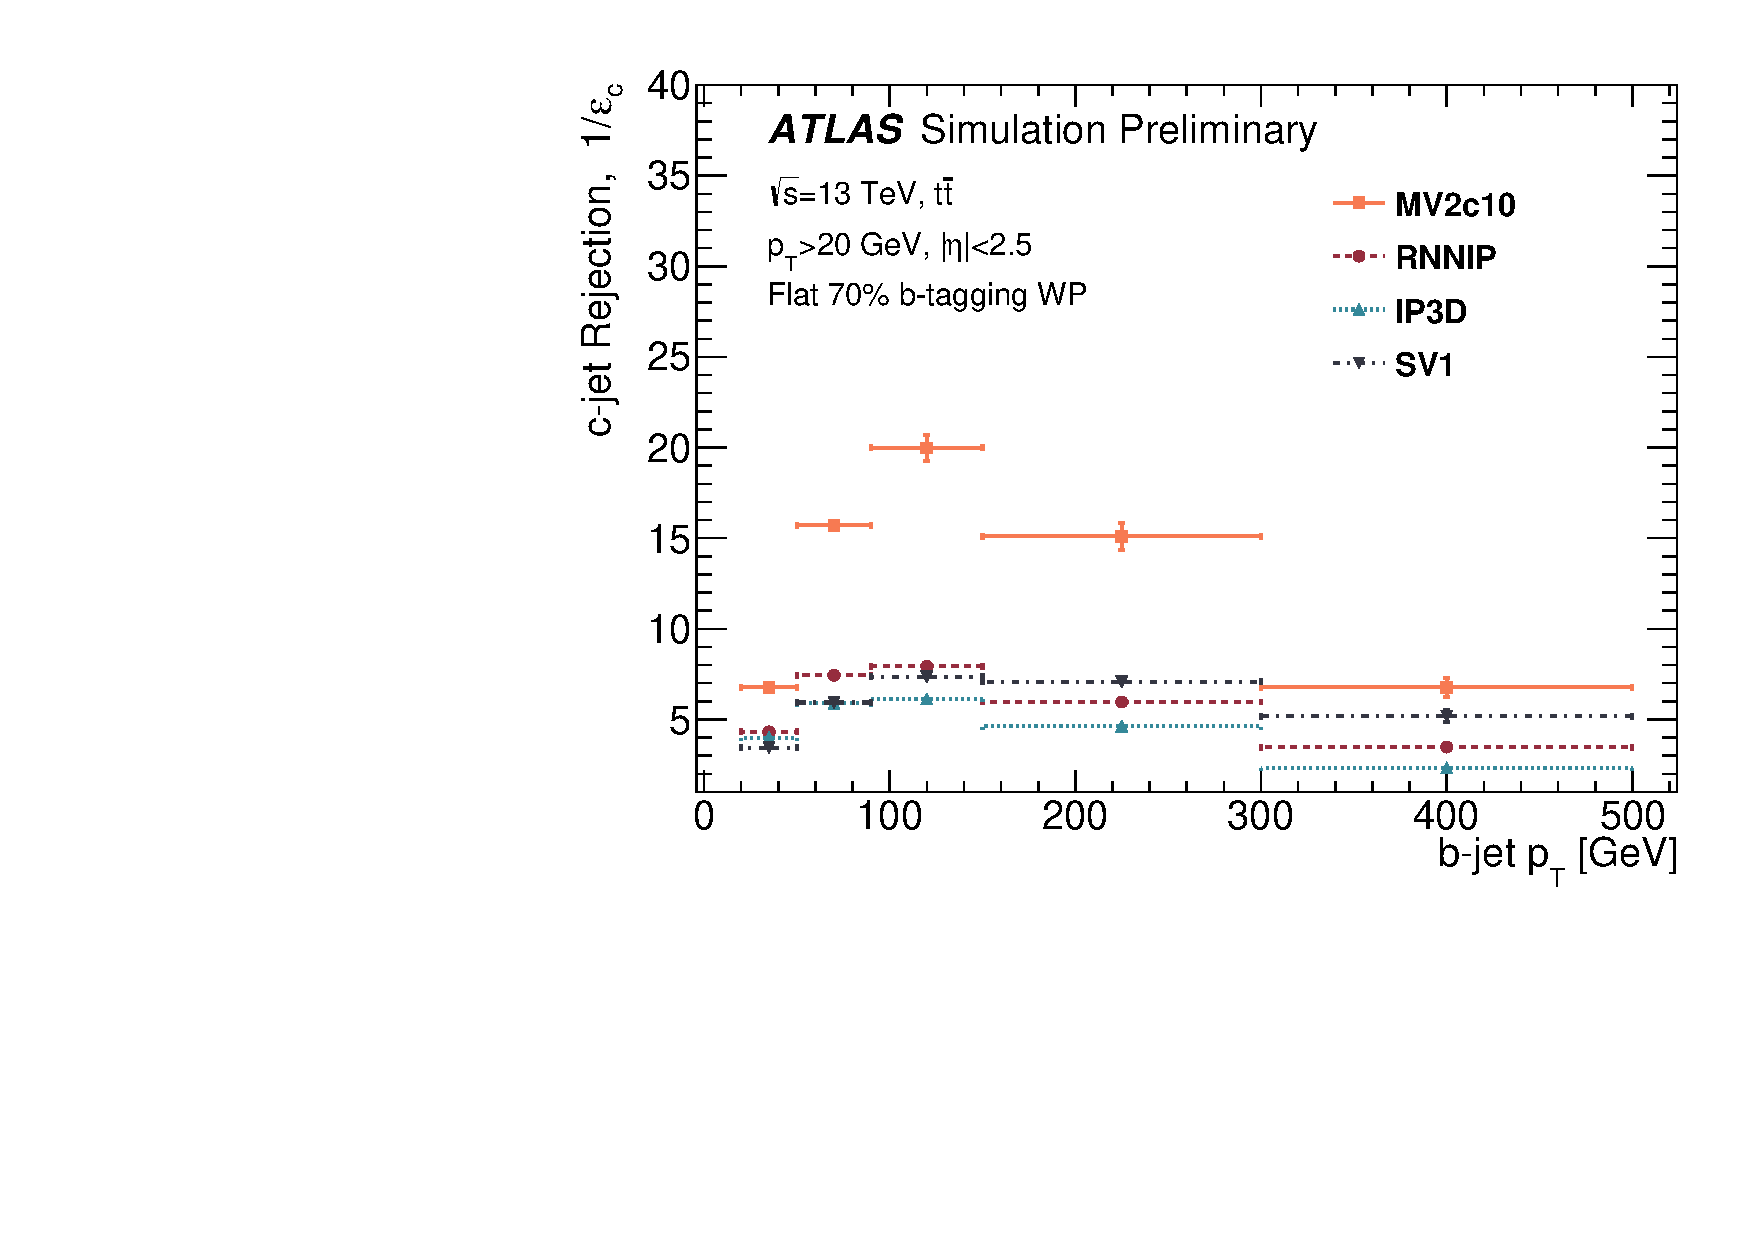
\includegraphics[width=0.41\linewidth]{\figpath/fig_06b}
%        } 
%        \caption{}
%        \label{fig:\jetdef-fig6}
%    \end{figure}
    
}
